\section{Opis}

Projekat se bavi sektorom prodaje u okviru poslovanje neke veleprodaje. Zaposleni u prodaje može biti komercijalista i menadžer. Komercijalista evidentira kupce i u kontaktu sa njima prima porudžbinu, recimo putem imejla. Tabela Kupac predstavlja pravno lice, dok tabela Kontakt osobe, predstavlja fizička lica sa kojima poslujemo u okviru određene firme.

Glavni deo baza predstavlja odnos specijalizavije tabele Dokument na Porudžbina,Ponuda,Otpremnica i Faktura. Dokument svaki ima posebne atribute, kao i svoje stavke, koje daju informacije o proizvodu i potrebnoj količini istog.

Porudžbinu evidentira komercijalista u kontaktu sa kupcem.
Zatim komercijalista sastavlja ponudu kupcu, uz eventualno prisustvo menadžera, koji može dati popust određeni, radi uspešnijeg nastavka saradnje. Tabela Izrađuje čuva podatke o zaposlenima koji učestvuju u sastavljanju određenog dokumenta. Ponuda sadrži za razliku od porudžbine sadrži cene, i detalje posla, kao što su način isporuke, rok isporuke, rok plaćanja, opciono kontinuitet isporuke (u sličaku da može roba iz više puta da se dostavi).

Ponuda može imati više otpremnica, u sličaju da je postignut dogovor oko kontinuiteta isporuke ili trenutno samo toliko možemo isporučiti. Otpremnica ne sadrži cene i ona se šalje magacinu za odvajanje robe. 

Na osnovu otpremnice se izrađuje faktura, koja naplaćuje kupcu robu koja će mu biti isporučena na osnovu otpremnice.

Rekurzivni odnos se ostvaruje preko tabele Proizvod, jer postoji proizvodi koji se prodaju,a sastoje se od postojećih proizvoda. Recimo pakovanja od vise komada, promocije, ili paketi lekova koji se često zajedno naručuju.


\subsection{Relacioni model}
\begin{itemize}
\item Zaposleni (idZaposleni*, ImePrezime, DatumZaposlenja, StručnaSprema, Fukcija, UgovorenaPlata)
\item Kupac (idKupac*, PIB, NazivFirme, TekuciRačun)
\item Kontakt osoba (idKontOsobe* ,idKupac*, ImePrezime, Telefon)
\item Dokument (idDokument*, VremeKreiranja, VremeIzmene, Status)

\item Izradjuje (Dokument\_idDokument*, Zaposleni\_idZaposleni*)

\item Porudžbina (idPorudzbina*, Kupac\_idKupac, DatumPorudzbine)

\item Proizvod (idProizvod*, Naziv, Cena)

\item Proizvod\_has\_Proizvod (idProizvod*, idProizvod1*)

\item Stavka (idDokumenta*, idProizvod*, Kolicina)

\item Ponuda (idPonuda*, idPorudžbina, DatumPonude, Cena, Popust, ProdajnaCena, Kontinuitet i broj isporuka, Način isporuke, Rok plaćanja)

\item Otpremnica (idOtpremnica*, idMagacina,Ponuda\_idPonuda)

\item Faktura (idFaktura*, idOtpremnica, Rok isporuke)
\end{itemize}

\subsection{Uslovi}
\begin{itemize}
\item Nezavisni eniteti: Zaposleni, Kupac, Porudžbina, Ponuda, Otpremnica, Faktura

\item Agregirani entiteti: Izradjuje

\item Rekurzivni odnos: Proizvod\_has\_Proizvod

\item Slabi entitet: Kontakt\_osoba

\item Generalizacija/Specijalizacija: Dokument -> Porudzbina,Ponuda,Otpremnica,Faktura

\end{itemize}

\clearpage

\begin{figure}[ht]
\centering
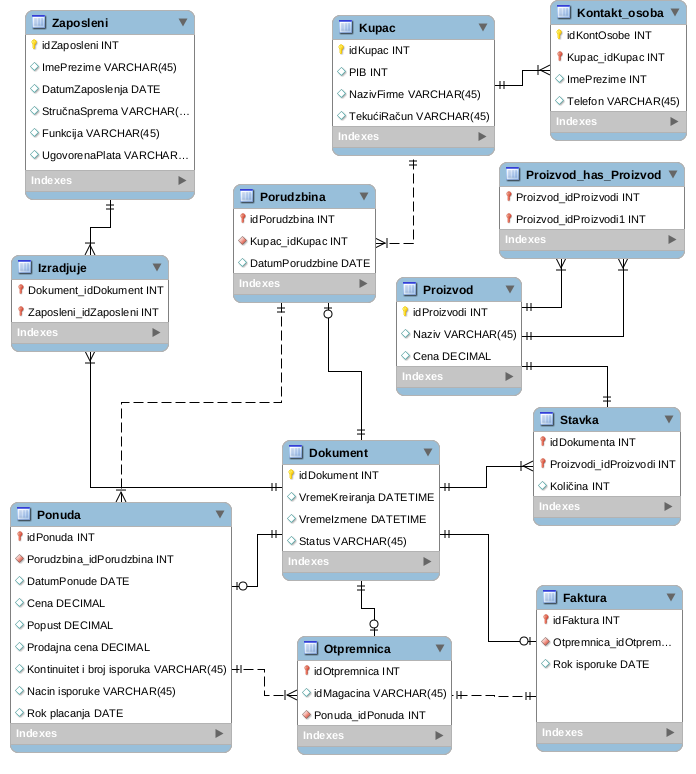
\includegraphics[width=160mm]{slike/er.png}%
\caption{EER dijagram}
\end{figure}

\clearpage